%================================================================
% TEMPLATE TUGAS AKHIR SARJANA (S1)
% IPB University
%
% Diadaptasi dari Template Word PPKI (Pedoman Penulisan Karya Ilmiah) Edisi ke-4
%
% Konversi dan adaptasi ke LaTeX oleh:
%   Raihan Putra Kirana
%   GitHub: https://github.com/raihanpka
%
% Versi: v1.0 (Mei 2026)
%
% Silakan gunakan, modifikasi, dan distribusikan secara bebas
% dengan tetap mencantumkan atribusi di atas.
%================================================================

\documentclass[12pt,a4paper,openany,twoside]{book}

%--------------------------------------------------------------
% # Encoding
% - T1        : Font encoding 8-bit, mendukung karakter Latin penuh
% - textcomp  : Simbol tambahan encoding TS1
% - utf8      : Input encoding Unicode, mendukung karakter Indonesia
% - babel     : Dukungan bahasa Indonesia (hyphenation, tanggal, dan lainnya)
%--------------------------------------------------------------
\usepackage[T1]{fontenc}
\usepackage{textcomp}
\usepackage[utf8]{inputenc}
\usepackage[indonesian, provide=*]{babel}

%--------------------------------------------------------------
% # Font
% - Times New Roman
% - mathptmx menyediakan Times Roman untuk teks dan matematika.
% - Alternatif untuk XeLaTeX atau LuaLaTeX dapat menggunakan:
%     \usepackage{fontspec}
%     \setmainfont{Times New Roman}
%--------------------------------------------------------------
\usepackage{mathptmx}

%--------------------------------------------------------------
% # Ukuran Halaman & Margin
% - A4: 21 x 29.7 cm
% - Kiri 4 cm (binding), Kanan 3 cm, Atas 3 cm, Bawah 3 cm
%--------------------------------------------------------------
\usepackage[
  a4paper,
  top=3cm,
  left=4cm,
  right=3cm,
  bottom=3cm,
  headheight=15pt
]{geometry}

%--------------------------------------------------------------
% # Spasi & Indentasi
%--------------------------------------------------------------
\usepackage{setspace}
\singlespacing                   % Spasi tunggal (sesuai template)
\usepackage{indentfirst}          % Indentasi paragraf pertama
\setlength{\parindent}{1cm}      % Indentasi awal paragraf ±1 cm
\setlength{\parskip}{0pt}        % Tidak ada jarak antar paragraf
\setlength{\textfloatsep}{12pt plus 2pt minus 2pt}  % Jarak float atas/bawah ke teks
\setlength{\intextsep}{8pt plus 2pt minus 2pt}    % Jarak float di tengah teks
\setlength{\floatsep}{8pt plus 2pt minus 2pt}      % Jarak antar-float

%--------------------------------------------------------------
% # Header & Footer (fancyhdr)
%--------------------------------------------------------------
\usepackage{fancyhdr}

% Halaman preliminari: nomor halaman romawi kecil, tengah atas
\fancypagestyle{frontmatter}{%
  \fancyhf{}
  \fancyhead[RO,LE]{\thepage}
  \renewcommand{\headrulewidth}{0pt}
  \renewcommand{\footrulewidth}{0pt}
}

% Halaman isi/bab: nomor halaman arab, kanan atas
\fancypagestyle{mainmatter}{%
  \fancyhf{}
  \fancyhead[RO,LE]{\thepage}
  \renewcommand{\headrulewidth}{0pt}
  \renewcommand{\footrulewidth}{0pt}
}

% Halaman plain (halaman pertama bab) = sama seperti mainmatter
\fancypagestyle{plain}{%
  \fancyhf{}
  \fancyhead[RO,LE]{\thepage}
  \renewcommand{\headrulewidth}{0pt}
  \renewcommand{\footrulewidth}{0pt}
}

%--------------------------------------------------------------
% # Format Judul Bab & Subbab (titlesec)
%--------------------------------------------------------------
\usepackage{titlesec}

% Bab utama : 14pt, tebal, rata tengah, dengan huruf kapital otomatis
% Format    : "I  PENDAHULUAN" (semua dalam satu baris)
\titleformat{\chapter}[block]
  {\centering\fontsize{14pt}{17pt}\selectfont\bfseries}
  {\thechapter\enspace}
  {0pt}
  {\MakeUppercase}
  []

% Jarak sebelum dan sesudah judul bab
\titlespacing*{\chapter}{0pt}{-30pt}{24pt}

% Subbab    : 12pt, tebal, rata kiri
\titleformat{\section}
  {\fontsize{12pt}{14pt}\selectfont\bfseries}
  {\thesection}
  {1em}
  {}
\titlespacing*{\section}{0pt}{12pt}{6pt}

% Sub-subbab: 12pt, tebal, rata kiri, lebih dalam
\titleformat{\subsection}
  {\fontsize{12pt}{14pt}\selectfont\bfseries}
  {\thesubsection}
  {1em}
  {}
\titlespacing*{\subsection}{0pt}{6pt}{3pt}

% Sub-sub-subbab: 12pt, tebal, rata kiri, lebih dalam lagi
\titleformat{\subsubsection}
  {\fontsize{12pt}{14pt}\selectfont\bfseries}
  {\thesubsubsection}
  {1em}
  {}
\titlespacing*{\subsubsection}{0pt}{6pt}{3pt}

%--------------------------------------------------------------
% # Penomoran Bab & Subbab
% Bab     : Romawi (I, II, III...)
% Subbab  : 1.1, 1.2, dst. (berurutan dengan nomor bab)
%--------------------------------------------------------------
\renewcommand{\thechapter}{\Roman{chapter}}
\renewcommand{\thesection}{\arabic{chapter}.\arabic{section}}
\renewcommand{\thesubsection}{\arabic{chapter}.\arabic{section}.\arabic{subsection}}
\renewcommand{\thesubsubsection}{\arabic{chapter}.\arabic{section}.\arabic{subsection}.\arabic{subsubsection}}

%--------------------------------------------------------------
% # Penomoran Gambar & Tabel
% Penomoran berurutan di seluruh dokumen (tidak reset per bab)
%--------------------------------------------------------------
\usepackage{chngcntr}
\counterwithout{figure}{chapter}
\counterwithout{table}{chapter}

%--------------------------------------------------------------
% # Keterangan Gambar & Tabel (caption)
% Format sesuai template IPB:
%   - Gambar 1 Judul gambar (di bawah gambar)
%   - Tabel 1 Judul tabel (di atas tabel)
%   - Tanpa titik dua, tanpa bold/italic pada label maupun judul
%   - Hanging indentation, baris lanjutan rata dengan awal judul
%   - Rata kiri (justified=false)
%--------------------------------------------------------------
\usepackage{caption}

% Format dasar
\DeclareCaptionFormat{ipbcap}{#1#2#3\par}
\DeclareCaptionLabelFormat{ipblabel}{#1~#2}  % "Gambar 1" / "Tabel 1"

\captionsetup{
  format        = hang,           % Hanging indent (baris lanjutan rata dengan judul)
  labelformat   = ipblabel,
  labelsep      = space,          % Tanpa titik dua, hanya spasi
  font          = normalsize,     % 12pt sama dengan teks
  labelfont     = {},             % Label tidak bold
  textfont      = {},             % Judul tidak bold maupun italic
  justification = justified,        % Rata kiri-kanan
  singlelinecheck = false,
  hangindent    = 0pt             % LaTeX akan otomatis pakai lebar label
}

\captionsetup[figure]{
  name     = Gambar,
  position = below,               % Caption di bawah gambar
  justification = justified,      % Caption panjang tetap rata kiri-kanan
  singlelinecheck = true          % Caption satu baris akan diposisikan ke tengah
}

\captionsetup[table]{
  name     = Tabel,
  position = above                % Caption di atas tabel
}

% Counter lampiran untuk caption
\newcounter{lampiran}
\renewcommand{\thelampiran}{\arabic{lampiran}}
\newcommand{\captionlampiran}[1]{%
  \refstepcounter{lampiran}%
  \par\noindent\hangindent=5.5em
  \textbf{}\makebox[5em][l]{Lampiran \thelampiran}#1\par
}

%--------------------------------------------------------------
% # Daftar Isi, Daftar Tabel, Daftar Gambar (tocloft)
%--------------------------------------------------------------
\usepackage{tocloft}

% Judul daftar isi
\renewcommand{\cfttoctitlefont}{\hfill\fontsize{14pt}{17pt}\selectfont\bfseries}
\renewcommand{\cftaftertoctitle}{\hfill}
\renewcommand{\cftlottitlefont}{\hfill\fontsize{14pt}{17pt}\selectfont\bfseries}
\renewcommand{\cftafterlottitle}{\hfill}
\renewcommand{\cftloftitlefont}{\hfill\fontsize{14pt}{17pt}\selectfont\bfseries}
\renewcommand{\cftafterloftitle}{\hfill}

% Entri bab di daftar isi (tidak bold, menggunakan font normal)
\renewcommand{\cftchapfont}{\normalfont}
\renewcommand{\cftchappagefont}{\normalfont}
\renewcommand{\cftchapleader}{\cftdotfill{\cftdotsep}}

% Indentasi entri di daftar isi
\setlength{\cftchapindent}{0pt}
\setlength{\cftsecindent}{1.5em}
\setlength{\cftsubsecindent}{3.5em}

% Jarak antar entri
\setlength{\cftbeforechapskip}{0pt}
\setlength{\cftbeforesecskip}{0pt}

% Format entri bab seperti "I  PENDAHULUAN"
\renewcommand{\cftchapaftersnum}{\enspace}

%--------------------------------------------------------------
% # Format Tabel
%--------------------------------------------------------------
\usepackage{booktabs}        % \toprule, \midrule, \bottomrule
\usepackage{array}           % Opsi kolom tambahan
\usepackage{tabularx}        % Tabel lebar fleksibel
\usepackage{multirow}        % Sel bergabung baris
\usepackage{longtable}       % Tabel panjang lintas halaman

%--------------------------------------------------------------
% # Format Gambar
%--------------------------------------------------------------
\usepackage{graphicx}
\usepackage{float}            % Opsi [H] untuk posisi gambar

%--------------------------------------------------------------
% # Format Matematika
%--------------------------------------------------------------
\usepackage{amsmath}
\usepackage{amssymb}

%--------------------------------------------------------------
% # Referensi & Sitasi
%--------------------------------------------------------------
\usepackage[authoryear,round,sort&compress]{natbib}
\setlength{\bibsep}{0pt}  % Tidak ada jarak ekstra antar referensi

%--------------------------------------------------------------
% # Hyperlink (harus dimuat terakhir)
%--------------------------------------------------------------
\usepackage[
  colorlinks=false,
  hidelinks,
  pdfauthor={Nama Mahasiswa},
  pdftitle={Judul Skripsi},
  pdfsubject={Skripsi S1 IPB},
  pdfkeywords={keyword1, keyword2}
]{hyperref}

%--------------------------------------------------------------
% # Paket tambahan untuk perbaikan tipografi, warna, URL, dan kontrol list
%--------------------------------------------------------------
\usepackage{microtype}      % Perbaikan tipografi otomatis
\usepackage{xcolor}         % Dukungan warna
\usepackage{url}            % Format URL
\usepackage{enumitem}       % Kontrol list/enumerate
\usepackage{hanging}        % Hanging indent untuk daftar pustaka manual


%==============================================================
% # TITIK MULAI DOKUMEN
%==============================================================
\begin{document}

%--------------------------------------------------------------
% # BAGIAN AWAL (PRELIMINARI)
%--------------------------------------------------------------
\frontmatter
\pagestyle{frontmatter}

%==============================================================
% HALAMAN JUDUL (COVER)
% Sesuaikan bagian bertanda [ISIAN] dengan data mahasiswa
%==============================================================

\begin{titlepage}
\thispagestyle{empty}
\begin{center}


\vspace*{1cm}

{\fontsize{14pt}{17pt}\selectfont\bfseries
JUDUL KARYA ILMIAH MAKSIMUM TIGA BARIS,\\
LIMA BELAS KATA TIDAK TERMASUK\\
KATA DEPAN DAN KATA SAMBUNG
}

\vspace{3cm}

{\fontsize{14pt}{17pt}\selectfont\bfseries
NAMA PENULIS
}

\vspace{6cm}

% Logo IPB tengah halaman

\includegraphics[width=2.5cm]{images/ipb_logo}

\vspace{4cm}

{\fontsize{14pt}{17pt}\selectfont\bfseries
NAMA DEPARTEMEN/PROGRAM STUDI\\
FAKULTAS/SEKOLAH\\
INSTITUT PERTANIAN BOGOR\\
BOGOR\\
20XX
}

\end{center}
\end{titlepage}

% Halaman kosong di balik cover (halaman ii - tidak bernomor)
\cleardoublepage

%==============================================================
% PERNYATAAN MENGENAI SKRIPSI DAN
% SUMBER INFORMASI SERTA PELIMPAHAN HAK CIPTA
%==============================================================

\chapter*{PERNYATAAN MENGENAI SKRIPSI DAN\\
SUMBER INFORMASI SERTA PELIMPAHAN HAK CIPTA}
% Halaman ini tidak dimasukkan ke Daftar Isi (tidak ada \addcontentsline)

\noindent
Dengan ini saya menyatakan bahwa skripsi dengan judul
``\textit{Judul Karya Ilmiah Tugas Akhir}''
adalah karya saya dengan arahan dari dosen pembimbing dan belum diajukan
dalam bentuk apa pun kepada perguruan tinggi mana pun.
Sumber informasi yang berasal atau dikutip dari karya yang diterbitkan
maupun tidak diterbitkan dari penulis lain telah disebutkan dalam teks
dan dicantumkan dalam Daftar Pustaka di bagian akhir skripsi ini.

Dengan ini saya melimpahkan hak cipta dari karya tulis saya kepada
Institut Pertanian Bogor.

\vspace{2cm}

\noindent
Bogor, Bulan Tahun 20XX

\vspace{2cm}

\noindent
Nama\\
NIM

%==============================================================
% ABSTRAK DAN ABSTRACT
% Satu halaman berisi keduanya, tanpa nomor halaman.
% Format sesuai PPKI IPB Edisi ke-4.
%==============================================================

\clearpage
\thispagestyle{empty}

% --- ABSTRAK (Bahasa Indonesia) ---
\begin{center}
{\fontsize{14pt}{17pt}\selectfont\bfseries ABSTRAK}
\end{center}

\vspace{6pt}

NAMA MAHASISWA. Judul Skripsi.
Dibimbing oleh NAMA PEMBIMBING 1 dan NAMA PEMBIMBING 2.

\vspace{12pt}

% --- ABSTRACT (Bahasa Inggris) ---
\begin{center}
{\fontsize{14pt}{17pt}\selectfont\bfseries ABSTRACT}
\end{center}

\vspace{6pt}

STUDENT NAME. Title of Thesis (skripsi).
Supervised by NAME of 1st SUPERVISOR and NAME of 2nd SUPERVISOR.

\vspace{12pt}

Narasi disusun dalam satu paragraf, isi tidak lebih dari 200 kata,
dan ditulis dalam satu halaman untuk abstrak dan abstract.
Abstrak memuat latar belakang permasalahan (tentatif), tujuan penelitian,
metode, hasil penelitian dengan penekanan pada temuan baru, dan implikasi
yang disajikan secara informatif dan faktual.
Tidak diperbolehkan mengacu pustaka, gambar, dan tabel.
Singkatan hanya dikenalkan jika masih digunakan lagi dalam bagian lain
Abstrak/Abstract.

\vspace{12pt}

\noindent
Kata kunci: ditulis dalam bahasa Indonesia, disusun berdasarkan abjad,
maksimum lima kata atau frasa

\vspace{6pt}

\noindent
\textit{Keywords}: ditulis dalam bahasa Inggris, disusun berdasarkan abjad,
maksimum lima kata atau frasa

%==============================================================
% LEMBAR PENGESAHAN / HALAMAN PERSETUJUAN
% Format sesuai template PPKI IPB Edisi ke-4
%==============================================================

\clearpage
\thispagestyle{empty}

\noindent
{\fontsize{12pt}{14pt}\selectfont
\begin{tabular}{@{}p{2.5cm}p{0.3cm}p{0.62\textwidth}@{}}
Judul Skripsi & : & Judul Karya Ilmiah Maksimum Tiga Baris, Lima Belas Kata Tidak Termasuk Kata Depan Dan Kata Sambung \\
Nama & : & Nama Lengkap \\
NIM  & : & NIM \\
\end{tabular}
}

\vspace{2cm}

\begin{center}
Disetujui oleh
\end{center}

\vspace{0.5cm}

\noindent
\begin{tabular}{@{}p{0.55\textwidth}@{}p{0.45\textwidth}@{}}
Pembimbing 1: & \\
\hspace{0.5cm}Nama lengkap dan gelar & \hfill\rule{4cm}{0.4pt} \\[1cm]
Pembimbing 2: & \\
\hspace{0.5cm}Nama lengkap dan gelar & \hfill\rule{4cm}{0.4pt} \\
\end{tabular}

\vspace{2cm}

\begin{center}
Diketahui oleh
\end{center}

\vspace{0.5cm}

\noindent
\begin{tabular}{@{}p{0.55\textwidth}@{}p{0.45\textwidth}@{}}
Ketua Program Studi: & \\ 
\hspace{0.5cm}Nama lengkap dan gelar & \hfill\rule{4cm}{0.4pt} \\
\hspace{0.5cm}NIP

\textit{(Atau pilih salah satu)} & \\

Ketua Departemen \ldots: & \\
\hspace{0.5cm}Nama lengkap dan gelar & \hfill\rule{4cm}{0.4pt} \\
\hspace{0.5cm}NIP & \\
\end{tabular}

\vfill

\noindent
\begin{tabular}{@{}p{0.5\textwidth}@{}p{0.5\textwidth}@{}}
Tanggal Ujian: & Tanggal Lulus: \\
{\fontsize{9pt}{11pt}\selectfont (tanggal pelaksanaan ujian)} &
{\fontsize{9pt}{11pt}\selectfont (tanggal penandatanganan oleh Dekan Fakultas/Sekolah \ldots)} \\
\end{tabular}

%==============================================================
% PRAKATA
%==============================================================

\chapter*{PRAKATA}

Puji dan syukur penulis panjatkan kepada Allah \textit{subhanaahu wa ta'ala}
atas segala karunia-Nya sehingga karya ilmiah ini berhasil diselesaikan.
Tema yang dipilih dalam penelitian yang dilaksanakan sejak bulan .... 20XX
sampai bulan .... 20XX ini ialah .........., dengan judul
``...........................................................................''.

Terima kasih penulis ucapkan kepada para pembimbing,
... (nama lengkap dan gelar) yang telah membimbing dan banyak memberi saran.
Ucapan terima kasih juga disampaikan kepada pembimbing akademik,
moderator seminar, dan penguji luar komisi pembimbing.
Di samping itu, penghargaan penulis sampaikan kepada
... (nama lengkap dan gelar dari lembaga/instansi/perusahaan yang telah memberi
izin penelitian), (nama dan gelar atau bapak/ibu jika tidak ada gelar)
beserta staf Laboratorium ..... dan seterusnya .... yang telah membantu
selama pengumpulan data.
Ungkapan terima kasih juga disampaikan kepada ayah, ibu, serta seluruh keluarga
(istri/suami/anak jika sudah menikah) yang telah memberikan dukungan,
doa, dan kasih sayangnya .... dan seterusnya.

Semoga karya ilmiah ini bermanfaat bagi pihak yang membutuhkan dan bagi
kemajuan ilmu pengetahuan.

\vspace{2cm}

\noindent
Bogor, Bulan Tahun

\vspace{1.5cm}

\noindent
\textit{Nama penulis}

%==============================================================
% DAFTAR ISI
%==============================================================
\renewcommand{\contentsname}{DAFTAR ISI}
\tableofcontents

\clearpage

%==============================================================
% DAFTAR TABEL
% (jika tabel hanya satu tidak perlu dibuat daftar)
%==============================================================
\renewcommand{\listtablename}{DAFTAR TABEL}
\addcontentsline{toc}{chapter}{DAFTAR TABEL}
\listoftables

\clearpage

%==============================================================
% DAFTAR GAMBAR
% (jika gambar hanya satu tidak perlu dibuat daftar)
%==============================================================
\renewcommand{\listfigurename}{DAFTAR GAMBAR}
\addcontentsline{toc}{chapter}{DAFTAR GAMBAR}
\listoffigures

\clearpage

%==============================================================
% DAFTAR LAMPIRAN
% (jika lampiran hanya satu tidak perlu dibuat daftar)
%==============================================================

\chapter*{DAFTAR LAMPIRAN}
\addcontentsline{toc}{chapter}{DAFTAR LAMPIRAN}

\noindent
\begin{enumerate}[label=\arabic*., leftmargin=2em]
  \item Lampiran 1 \enspace Rata-rata dan simpangan baku beberapa sifat fisik dan kimia
        tanah dari 78 contoh tanah di Kebun Percobaan Ciheuleut
        \dotfill \pageref{lamp:tanah}

  \item Lampiran 2 \enspace Umur, indeks luas daun, dan hasil biji kering jagung yang
        ditanam pada lima ketinggian tempat
        \dotfill \pageref{lamp:jagung}
\end{enumerate}


%--------------------------------------------------------------
% # BAGIAN INTI (BAB)
%--------------------------------------------------------------
% Hindari halaman kosong di transisi frontmatter -> mainmatter saat twoside.
\let\origcleardoublepage\cleardoublepage
\let\cleardoublepage\clearpage
\mainmatter
\let\cleardoublepage\origcleardoublepage
\pagestyle{mainmatter}

%==============================================================
% BAB I  PENDAHULUAN
%==============================================================

\chapter{PENDAHULUAN}

Bab pendahuluan memuat latar belakang atau alasan kuat dilakukannya penelitian,
tujuan, dan hipotesis jika ada.
Di dalam pendahuluan dijelaskan pula perumusan atau pendekatan penyelesaian masalah
dan alasan pemilihan metode yang digunakan.
Bergantung pada proses perumusan masalah penelitian, bagian Kerangka Pikir dan
Hipotesis dapat ditulis di sini, tidak ditulis dalam bab tersendiri.

Paparan tidak berbelit-belit atau dimulai dengan latar belakang yang terlalu umum.
Pernyataan mengenai apa yang diteliti dan apa yang diharapkannya diawali dengan
pemikiran logis.
Tujuan penelitian ditulis di bagian akhir bab ini dengan memilih kata kerja yang
hasilnya dapat diukur dan dilihat, seperti:
\textit{menguraikan, menerangkan, membuktikan, menjajaki, menguji, membuktikan,
atau menerapkan suatu gejala, konsep atau dugaan}, atau bahkan
\textit{membuat suatu prototipe}.
Jangan menggunakan kata kerja mengetahui atau memahami.

Untuk tesis/disertasi dengan pola rangkaian penelitian, dapat dituliskan telaah
pustaka secara umum.
Kebaruan (\textit{novelty}) merupakan hal penting yang harus jelas tersurat atau
tersirat dalam disertasi.
Hal ini berarti penelitian disertasi bukan sekadar mengulang atau mengadaptasi
penelitian yang telah dikerjakan oleh orang lain.
Kebaruan dapat berupa penggunaan metode baru atau pendekatan baru untuk menelaah
suatu permasalahan.


%--------------------------------------------------------------
\section{Latar Belakang}
%--------------------------------------------------------------

Latar Belakang memuat ulasan singkat mengapa penelitian perlu dilakukan.
Uraian dimulai dengan hal yang unik, fakta, masalah, dan pendapat yang mendasari
dilakukannya penelitian.
Di dalamnya diuraikan juga alasan teoretis dan alasan praktis dari perlunya
penelitian dilakukan, dan bagaimana masalah tersebut dapat dipecahkan dan manfaat
dari penyelesaian masalah.


%--------------------------------------------------------------
\section{Rumusan Masalah}
%--------------------------------------------------------------

Berbekalkan latar belakang dan kerangka pikir, masalah yang diteliti dapat
dirumuskan.
Masalah yang dirumuskan harus jelas dan fokus pada kata kunci utama yang unik.
Dalam merumuskan masalah, deskripsi lokasi studi terutama keunikannya sudah
termasuk dalam pertimbangan.
Untuk memperjelas perumusan masalah, dapat juga dibuat beberapa pertanyaan yang
hendak dijawab dalam penelitian itu.
Dalam uraian harus tercakup pendekatan yang digunakan dalam perumusan masalah.
Untuk membantu mengikuti alur pikir secara skematis, dapat juga dibuat bagan alir
kerangka proses dan rumusan masalah serta pencapaian tujuan penelitian.


%--------------------------------------------------------------
\section{Tujuan}
%--------------------------------------------------------------

Pernyataan tujuan penelitian ialah pernyataan singkat dan jelas tentang tujuan
yang akan dicapai sebagai upaya pemecahan masalah maupun memahami gejala
(fenomena) yang dijelaskan dalam latar belakang.
Gunakan kata kerja yang hasilnya dapat diukur.
Bila ada atau memungkinkan, dapat ditulis manfaat atau kegunaan hasil penelitian
bagi kepentingan pengembangan ipteks, pertimbangan dalam mengambil kebijakan,
kepentingan profesi maupun masyarakat pada umumnya.

%--------------------------------------------------------------
% CONTOH GAMBAR
% - Gambar ditempatkan dengan [H] atau [htbp]
% - Caption: di bawah gambar, format "Gambar N Judul"
% - Tanpa bold, tanpa titik dua, hanging indent otomatis
%--------------------------------------------------------------

\begin{figure}[H]
  \centering
  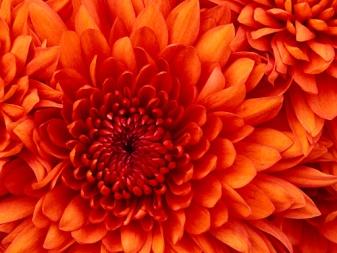
\includegraphics[width=0.5\textwidth]{images/contoh_gambar1}
  \caption{Contoh gambar}
  \label{fig:contoh_gambar1}
\end{figure}


%--------------------------------------------------------------
\section{Manfaat}
%--------------------------------------------------------------

Isi manfaat penelitian menjelaskan kontribusi penelitian terhadap pengembangan
ilmu pengetahuan dan teknologi serta manfaat praktisnya bagi masyarakat
\citep{Widowati2020}.

%--------------------------------------------------------------
% CONTOH TABEL
% Panduan tabel IPB:
% - Caption selalu di atas tabel
% - Format "Tabel N Judul tabel" (tanpa titik dua, tanpa bold)
% - Hanging indent: baris lanjutan rata dengan awal judul
% - Gaya three-line: \toprule, \midrule, \bottomrule (booktabs)
% - Tidak ada garis vertikal
% - Tidak ada garis horizontal internal kecuali setelah header
% - Catatan kaki tabel menggunakan notasi superskrip huruf kecil
%   dan ditulis di bawah tabel dengan \tabularnote atau manual
%--------------------------------------------------------------

\begin{table}[H]
  \caption{Tingkat kekerasan dan kandungan gula buah pisang ambon
           pada suhu simpan yang berbeda dan pemberian putresina}
  \label{tab:pisang_ambon}
  \centering
  \  % Tabel ukuran agak lebih kecil jika konten padat
  \begin{tabular}{lcccccc}
    \toprule
    \multirow{2}{*}{Perlakuan}
      & \multicolumn{6}{c}{Kekerasan buah dan kandungan gula pada hari ke-} \\
    \cmidrule(lr){2-7}
      & \multicolumn{2}{c}{0} & \multicolumn{2}{c}{7} & \multicolumn{2}{c}{14} \\
    \cmidrule(lr){2-3}\cmidrule(lr){4-5}\cmidrule(lr){6-7}
      & Keras$^{\,\mathrm{a}}$ & Gula & Keras$^{\,\mathrm{a}}$ & Gula
      & Keras$^{\,\mathrm{a}}$ & Gula \\
    \midrule
    \multicolumn{7}{l}{\textit{Suhu simpan}} \\
    \quad 15 ºC  & 10.20a & 0.38a & 13.40a & 0.56a & 11.83a & 0.73a \\
    \quad 28 ºC  & 10.64a & 0.55a & 14.22a & 1.82a & 88.43b & 14.41b \\
    \multicolumn{7}{l}{\textit{Putresina}} \\
    \quad Dengan putresina  & 11.07a & 0.53a & 13.23a & 0.87a & 21.19a & 6.98a \\
    \quad Tanpa putresina   & 10.76a & 0.40a & 14.40a & 1.52a & 41.82b & 6.91a \\
    \bottomrule
  \end{tabular}
  % Catatan kaki tabel: rata kiri, ukuran normal, di bawah garis bawah
  \begin{minipage}{\linewidth}
    \vspace{2pt}
    \footnotesize
    $^{\mathrm{a}}$Angka-angka pada kolom yang sama yang diikuti oleh huruf yang
    sama tidak berbeda nyata pada taraf uji 5\% (uji selang berganda Duncan).
  \end{minipage}
\end{table}


%--------------------------------------------------------------
\section{Ruang Lingkup (opsional)}
%--------------------------------------------------------------

Bagian ini menjelaskan batasan dan ruang lingkup penelitian yang dilakukan
agar pembaca dapat memahami cakupan serta keterbatasan studi.

% Contoh gambar dengan judul panjang lebih dari satu baris.
% Baris kedua otomatis dimulai tepat di bawah huruf pertama judul (hanging indent).

\begin{figure}[H]
  \centering
  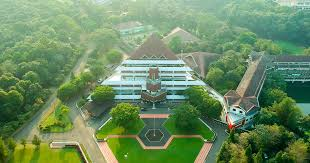
\includegraphics[width=0.7\textwidth]{images/contoh_gambar2}
  \caption{Contoh judul gambar lebih dari satu baris maka baris kedua
           dimulai tepat di bawah huruf pertama judul gambar}
  \label{fig:contoh_gambar2}
\end{figure}


%--------------------------------------------------------------
\section{Hipotesis (opsional)}
%--------------------------------------------------------------

Hipotesis dapat ditulis secara eksplisit atau tersirat sesuai bidang ipteks
yang relevan.
Hipotesis dapat menjadi bagian dari pendahuluan (untuk bidang eksakta atau
kajian eksperimental), atau merupakan bagian akhir dari tinjauan pustaka
(untuk bidang sosial dan ekonomi).

%==============================================================
% BAB II  TINJAUAN PUSTAKA (OPSIONAL)
%==============================================================

\chapter{TINJAUAN PUSTAKA (OPSIONAL)}

Pustaka yang digunakan dalam bab ini ialah acuan primer, diutamakan artikel
jurnal dan paten yang relevan dengan bidang yang diteliti, terkini, dan asli
(\textit{state of the art}).
Diktat dan buku ajar tidak termasuk acuan primer.
Tinjauan pustaka memuat telaah singkat, jelas, dan sistematis tentang kerangka
teoretis, kerangka pikir, temuan, postulat-postulat, prinsip, asumsi, dan
hasil-hasil penelitian yang relevan yang melandasi masalah penelitian atau
gagasan guna menggali pemahaman mengenai masalah penelitian dan pemecahan
masalahnya.
Oleh karena itu, dari tinjauan pustaka harus dapat diturunkan kerangka pikir,
hipotesis penelitian, dan metode penelitian.

%--------------------------------------------------------------
% CONTOH TABEL KEDUA (lanjutan sequential dari Tabel 1)
% Tabel ini menunjukkan cara tabel dengan baris subgrup dan
% catatan kaki superskrip.
%--------------------------------------------------------------

\begin{table}[htbp]
  \caption{Tingkat kekerasan buah pisang raja pada suhu simpan yang berbeda
           dan pemberian putresina}
  \label{tab:pisang_raja}
  \centering
  \begin{tabular}{lcccc}
    \toprule
\multirow{3}{*}{Perlakuan}
  & \multicolumn{4}{c}{Kekerasan buah dan kandungan gula pada hari ke-} \\
\cmidrule(lr){2-5}
  & 0 &  & 7 & 14 \\
\midrule
  & \multicolumn{4}{c}{Kekerasan buah (mm 50 g$^{-1}$ detik$^{-1}$)$^{\mathrm{a}}$} \\
    \multicolumn{5}{l}{\textit{Suhu Simpan}} \\
    \quad 15 ºC              & 9.20a  &  & 13.40a & 11.83a \\
    \quad 28 ºC              & 10.64a &  & 11.22a & 80.43b \\
    \multicolumn{5}{l}{\textit{Putresina}} \\
    \quad Dengan putresina   & 12.07a &  & 13.23a & 11.19a \\
    \quad Tanpa putresina    & 10.76a &  & 14.41a & 41.12b \\
    \bottomrule
  \end{tabular}
  \begin{minipage}{\linewidth}
    \vspace{2pt}
    \footnotesize
    $^{\mathrm{a}}$Angka-angka pada kolom yang sama yang diikuti oleh huruf yang
    sama tidak berbeda nyata pada taraf uji 5\% (uji selang berganda Duncan).
  \end{minipage}
\end{table}


%--------------------------------------------------------------
\section{Contoh Subbab}
%--------------------------------------------------------------

% --------------------------------------------------------------
\subsection{Contoh Sub-subbab}
% --------------------------------------------------------------

Berikut adalah contoh sub-subbab. Pada sub-subbab ini posisi paragraf lebih menjorok dari paragraf di subbab

%--------------------------------------------------------------
\section{Contoh Subbab2}
%--------------------------------------------------------------

Contoh tulisan
%==============================================================
% BAB III  METODE
%==============================================================

\chapter{METODE}

Bab ini dapat diawali dengan kerangka pendekatan studi.
Metode penelitian dapat berupa percobaan laboratorium, percobaan lapangan,
dan survei lapangan yang dirancang sesuai dengan tujuan atau jenis penelitian,
seperti: eksploratif, deskriptif, koreksional, kausal, komparatif, eksperimen,
tindakan (\textit{action research}), pemodelan, analisis suatu teori, atau
kombinasi dari berbagai jenis penelitian tersebut.
Untuk penelitian yang menggunakan metode kualitatif, jelaskan pendekatan yang
digunakan, proses pengumpulan dan analisis informasi, dan proses penafsiran
hasil penelitian.
Maksud dari perincian ini ialah untuk menjamin keterulangan hasil.


%--------------------------------------------------------------
\section{Waktu dan Tempat}
%--------------------------------------------------------------

%--------------------------------------------------------------
\section{Alat dan Bahan}
%--------------------------------------------------------------

%--------------------------------------------------------------
\section{Prosedur Kerja}
%--------------------------------------------------------------

%--------------------------------------------------------------
\section{Analisis Data}
%--------------------------------------------------------------


%==============================================================
% BAB IV  HASIL DAN PEMBAHASAN
%==============================================================

\chapter{HASIL DAN PEMBAHASAN}

Dalam penulisan hasil dan pembahasan dapat dipisah sebagai bab Hasil dan bab
Pembahasan, atau digabung menjadi bab Hasil dan Pembahasan.
Pemisahan atau penggabungan kedua bab ini bergantung pada bidang studi,
atau sesuai dengan arahan pembimbing.

% Jika dipisah, judul bab diganti:
%   \chapter{HASIL}
% dan file baru:
%   \chapter{PEMBAHASAN}


%--------------------------------------------------------------
\section{Hasil}
%--------------------------------------------------------------

Sajikan hasil penelitian secara sistematis.
Tabel dan gambar digunakan untuk mempermudah pembacaan data.
Setiap tabel dan gambar dirujuk dalam teks sebelum atau sesudah kemunculannya,
misalnya: (Tabel~\ref{tab:pisang_ambon}) atau (Gambar~\ref{fig:contoh_gambar1}).

Penulisan satuan mengikuti sistem SI.
Contoh penulisan satuan dalam teks: kekerasan buah diukur dalam
mm 50 g$^{-1}$ detik$^{-1}$ \citep{Kochel2005}.


%--------------------------------------------------------------
\section{Pembahasan}
%--------------------------------------------------------------

Pembahasan mengaitkan hasil penelitian dengan teori, hipotesis, dan hasil
penelitian sebelumnya.
Argumentasi penulis harus jelas dan didukung oleh data.
Kebaruan atau temuan penting ditekankan di bagian ini \citep{Onlamoon2010}.

Jangan hanya mengulang hasil; jelaskan mengapa hasil tersebut terjadi dan
apa artinya dalam konteks bidang ilmu.
Gunakan pustaka yang relevan untuk mendukung interpretasi.

%==============================================================
% BAB V  SIMPULAN DAN SARAN
%==============================================================

\chapter{SIMPULAN DAN SARAN}


%--------------------------------------------------------------
\section{Simpulan}
%--------------------------------------------------------------

Simpulan merupakan jawaban dari tujuan yang sudah ditentukan dan tidak
dimaksudkan sebagai ringkasan hasil.
Dalam Simpulan, penulis harus dan hanya menjawab masalah dan tujuan penelitian
yang telah dirumuskan pada Pendahuluan.
Simpulan merupakan generalisasi dari hasil penelitian dan argumentasi penulis,
atau pernyataan singkat yang merupakan hakikat dari bab Hasil dan Pembahasan
atau hasil pengujian berbagai hipotesis yang berkaitan.

Simpulan merupakan hasil penelitian yang boleh jadi telah dikemukakan dalam
perumusan masalah dan telah diberi jawaban sementara berupa hipotesis.
Dalam menulis simpulan, penulis harus membedakan dugaan, temuan, dan simpulan
hasil studi.
Pernyataan simpulan harus dilakukan secara cermat dan hati-hati.
Penyampaian simpulan ini dapat dilakukan sebanyak 3 kali, yakni dalam
Pembahasan, Simpulan, dan Abstrak sehingga diperlukan kecermatan untuk
menyajikannya dengan ungkapan yang berbeda-beda.


%--------------------------------------------------------------
\section{Saran}
%--------------------------------------------------------------

Saran seyogianya mengarah ke implikasi atau tindakan lanjutan yang harus
dilakukan sehubungan dengan temuan atau simpulan penulis.
Saran yang dikemukakan harus berkaitan dengan pelaksanaan atau hasil penelitian.
Dengan demikian saran ini mengemukakan hal-hal yang perlu diteliti lebih lanjut
terutama untuk memperbaiki kelemahan atau kekurangan dalam penelitian yang
dilakukan atau perbaikan asumsi yang diambil sehingga didapatkan hasil yang
lebih baik.
Jadi, saran tersebut harus diuraikan secara spesifik.
Jangan menyarankan hal-hal yang tidak dianalisis dan dibahas dalam penelitian
serta terkesan menggurui atau memuaskan keinginan peneliti.
Untuk penelitian yang berkaitan dengan permasalahan kebijakan, tidak perlu
menyarankan kebijakan yang tidak berkaitan dengan hasil penelitian.


%--------------------------------------------------------------
% # BAGIAN AKHIR
%--------------------------------------------------------------
% Catatan: \backmatter menonaktifkan penomoran bab di book class.
% Meskipun begitu, Chapter* digunakan agar tidak dapat nomor, 
% tapi halaman tetap urut dan fancyhdr tetap berjalan.
\backmatter
\pagestyle{mainmatter}

%==============================================================
% DAFTAR PUSTAKA
% Gaya sitasi IPB: author-year (Harvard), urut alfabet
% Format: Penulis Tahun. Judul. Jurnal. Vol(No):Hal. doi:...
%
% Catatan penting:
% - Nama penulis: Nama belakang + inisial depan (tanpa koma pemisah)
% - Tahun setelah nama penulis
% - Judul artikel: huruf kapital hanya kata pertama
% - Judul jurnal: italic
% - Semua penulis disebutkan (et al. hanya dalam teks jika >2 penulis)
%==============================================================

\chapter*{DAFTAR PUSTAKA}
\addcontentsline{toc}{chapter}{DAFTAR PUSTAKA}

% Aktifkan BibTeX agar perintah \citep{...} dari natbib dapat di-resolve.
% Natbib biasanya membuat heading bibliografi sendiri, jadi dimatikan agar
% heading tetap mengikuti format "DAFTAR PUSTAKA" di atas.
\renewcommand{\bibsection}{}
\bibliographystyle{ipb}
\bibliography{refs/daftar_pustaka}

%==============================================================
% LAMPIRAN
%==============================================================

% Halaman standalone judul "LAMPIRAN" di tengah halaman
\clearpage
\vspace*{\fill}
\begin{center}
  {\fontsize{14pt}{17pt}\selectfont\bfseries LAMPIRAN}
\end{center}
\vspace*{\fill}
\addcontentsline{toc}{chapter}{LAMPIRAN}

%--------------------------------------------------------------
% LAMPIRAN 1 (halaman tersendiri)
%--------------------------------------------------------------
\clearpage

\refstepcounter{lampiran}
\addcontentsline{lamp}{lampiran}{\protect\numberline{\thelampiran}Lampiran 1\enspace Rata-rata dan simpangan baku beberapa sifat fisik dan kimia tanah dari 78 contoh tanah di Kebun Percobaan Ciheuleut}
\label{lamp:tanah}

% Caption lampiran: di atas tabel, dengan format "Lampiran N Judul"
\noindent\hangindent=5.6em
\makebox[5.4em][l]{\textbf{Lampiran \thelampiran}}%
Rata-rata dan simpangan baku beberapa sifat fisik dan kimia tanah dari
78 contoh tanah di Kebun Percobaan Ciheuleut

\vspace{4pt}

\centering
\begin{tabular}{lcc}
  \toprule
  Sifat
    & Rata-rata
    & Simpangan baku \\
  \midrule
  Pasir (\%)                        & 47.66 & 23.81 \\
  Lempung (\%)                      & 21.80 & 11.94 \\
  Liat (\%)                         & 30.72 & 18.09 \\
  C-organik (\%)                    & 0.61  & 0.57  \\
  Rapatan isi (mg m$^{-3}$)         & 1.43  & 0.16  \\
  KTK (mek 100 g$^{-1}$ tanah)$^{\mathrm{a}}$
                                    & 18.08 & 17.09 \\
  KAT pada KL (g g$^{-1}$)         & 23.62 & 10.80 \\
  KAT pada TLP (g g$^{-1}$)        & 11.11 & 9.05  \\
  \bottomrule
\end{tabular}

\begin{minipage}{0.85\textwidth}
  \vspace{3pt}
  \footnotesize
  $^{\mathrm{a}}$Banyaknya 70 contoh tanah; KTK: kapasitas tukar kation,
  KAT: kadar air tanah, KL: kapasitas lapang, TLP: titik layu permanen.
\end{minipage}

\clearpage

%--------------------------------------------------------------
% LAMPIRAN 2
%--------------------------------------------------------------

\refstepcounter{lampiran}
\addcontentsline{lamp}{lampiran}{\protect\numberline{\thelampiran}Lampiran 2\enspace Umur, indeks luas daun, dan hasil biji kering jagung yang ditanam pada lima ketinggian tempat}
\label{lamp:jagung}

\noindent\hangindent=5.6em
\makebox[5.4em][l]{\textbf{Lampiran \thelampiran}}%
Umur, indeks luas daun, dan hasil biji kering jagung yang ditanam pada
lima ketinggian tempat

\vspace{4pt}

\noindent
\begin{tabular}{cccc}
  \toprule
  Ketinggian (m dpl) & Umur (hari) & Indeks luas daun & Hasil (ton ha$^{-1}$) \\
  \midrule
  856 & 115 & 3.10 & 5.69 \\
  605 & 106 & 3.09 & 5.43 \\
  400 & 100 & 2.47 & 4.80 \\
  210 &  93 & 2.46 & 4.25 \\
   10 &  88 & 2.12 & 4.03 \\
  \bottomrule
\end{tabular}

%==============================================================
% RIWAYAT HIDUP
%==============================================================

\chapter*{RIWAYAT HIDUP}
\addcontentsline{toc}{chapter}{RIWAYAT HIDUP}

Penulis dilahirkan di kota .... pada tanggal bulan tahun sebagai anak ke ...
dari pasangan bapak ... dan ibu ...
Pendidikan sekolah menengah atas (SMA) ditempuh di sekolah ..., dan lulus pada
tahun ....
Pada tahun ..., penulis diterima sebagai mahasiswa program sarjana (S-1) di
Program Studi/Fakultas/Sekolah ... di IPB.

Selama mengikuti program S-1, penulis aktif menjadi ... (riwayat dan pengalaman
organisasi, asisten akademik, dan sebagainya).
Penulis juga pernah mengikuti lomba karya ... (riwayat kegiatan ilmiah)
memperoleh atau pernah terpilih sebagai ... (riwayat prestasi akademik).


\end{document}
